\documentclass[epsfig,10pt,fullpage]{article}

\newcommand{\LabNum}{1}
\newcommand{\CommonDocsPath}{../../../../common/docs}
\addtolength{\textwidth}{1.5in}
\addtolength{\oddsidemargin}{-0.75in}
\addtolength{\topmargin}{-0.75in}
\addtolength{\textheight}{1.5in}
\addtolength{\evensidemargin}{0.75in}
\setlength\parindent{0pt}
\raggedbottom

\usepackage{ae,aecompl}
\usepackage{epsfig,float,times}
\usepackage[hypcap]{caption}
\usepackage[pdftex, colorlinks]{hyperref}
\usepackage{graphicx}
\usepackage[usenames, dvipsnames]{color}
\usepackage{rotating}
\usepackage{tikz}
\usetikzlibrary{automata,positioning}
\usepackage{placeins}

\widowpenalty 10000
\clubpenalty 10000

\newcommand{\red}[1]{{\color{red}\sf{#1}}}
\newcommand{\green}[1]{{\color{green}\sf{#1}}}
\newcommand{\blue}[1]{{\color{blue}\sf{#1}}}
\definecolor{PineGreen}{rgb}{0.0, 0.47, 0.44}
\definecolor{ForestGreen}{rgb}{0.13, 0.55, 0.13}
\definecolor{Brown}{rgb}{0.59, 0.29, 0.0}

\newcommand{\UPDatePublished}{Oct 2021}
\newcommand{\versnum}{21.1} %version number quartus/AMP
\newcommand{\quartusname}{Quartus\textsuperscript{\textregistered} Prime}	
\newcommand{\UPTextBar}{For \quartusname{} \versnum{}}
\newcommand{\thisyear}{2021 } %for copyright
\newcommand{\company}{FPGAcademy.org}
\newcommand{\longteamname}{FPGAcademy.org}
\newcommand{\teamname}{FPGAcademy}
\newcommand{\website}{FPGAcademy.org}

\newcommand{\productAcronym}{AMP}
\newcommand{\productNameShort}{Monitor Program}

\newcommand{\productNameMedTM}{A Monitor Program}
\newcommand{\productNameMed}{A Monitor Program}

%\newcommand{\headerLogoFilePath}[1]{#1/FPGAcademy.png}

% listings is a package that supports encapsulating source code in LaTeX conveniently
\usepackage{listings}

\def\expandparam\lstinputlisting[#1]#2{\edef\tmp{\noexpand\lstinputlisting[#1]{#2}}\tmp}

%%%%%%%%%%%%%%%%%%%% Source Code Formatting %%%%%%%%%%%%%%%%%%%%
\definecolor{globalCommentColour}{rgb}{0.588,0.588,0.588}

%%%%%%%%%%%%%%%%%%%%%%%%%%%%%%%%%%%%%%%%%%%%%%%%%%%%
% Defining language style
% NiosII ASM
\lstdefinelanguage[NiosII]{Assembler} {
  morekeywords={add, addi, and, andhi, andi, beq, bge, bgeu, bgt, bgtu, ble,  bleu, blt, bltu, bne, br, break,
  bret, call, callr, cmpeq, cmpeqi, cmpge, cmpgei, cmpgeu, cmpgeui, cmpgt, cmpgti, cmpgtu, cmpgtui, cmple,
  cmplei, cmpleu, cmpleui, cmplt, cmplti, cmpltu, cmpltui, cmpne, cmpnei, custom, div, divu, eret, flushd,
  flushda, flushi, flushp, initd, initda, initi, jmp, jmpi, ldb, ldbio, ldbu, ldbuio, ldh, ldhio, ldhu, ldhuio,
  ldw, ldwio, mov, movhi, movi, movia, movui, mul, muli, mulxss, mulxsu, mulxuu, nextpc, nop, nor, or, orhi, ori,
  rdctl, rdprs, ret, rol, roli, ror, sll, slli, sra, srai, srl, srli, stb, stbio, sth, sthio, stw, stwio,
  sub, subi, sync, trap, wrctl, wrtcl, wrprs, xor, xori, xorhi, xori},
  morekeywords=[2]{.abort, .ABORT, .align, .app-file, .ascii, .asciz, .balign, .byte, .comm, .data, .def,
  .desc, .dim, .double, .eject, .else, .end, .endef, .endif, .equ, .equiv, .err, .extern, .file, .fill, .float,
  .global, .globl, .hword, .ident, .if, .include, .int, .irp, .irpc, .lcomm, .lflags, .line, .linkonce, .ln,
  .list, .long, .macro, .mri, .nolist, .octa, .org, .p2align, .psize, .quad, .rept, .sbttl, .scl, .section,
  .set, .short, .single, .size, .sleb128, .skip, .space, .stadb, .stabn, .stabs, .string, .symver, .tag,
  .text, .title, .type, .val, .uleb128, .word},
  morekeywords=[3]{et, bt, gp, sp, fp, ea, sstatus, ra, pc, status, estatus, bstatus, ienable, ipending, cpuid,
  exception, pteaddr, tlbacc, tlbmisc, eccinj, badaddr, config, mpubase, mpuacc},
  sensitive=t,
  alsoletter=.,
  morestring=[b]",
  morecomment=[s]{/*}{*/},
  morecomment=[l]\#,
}[keywords,comments,strings]
   
%% NOTE: morekeywords=[2] are GNU directives.
   
\definecolor{niosInstructionColour}{rgb}{0.000,0.608,0.000}
\definecolor{niosDirectiveColour}{rgb}{0.000,0.000,0.902}
\definecolor{niosSpecialRegColour}{rgb}{0.000,0.000,0.000}
\definecolor{niosStringColour}{rgb}{0.808,0.482,0.000}
   
%% NOTE: To make bold use: =\bfseries\color{<colour>}
\lstdefinestyle{defaultNiosStyle} {
  language=[NiosII]{Assembler},
  stringstyle=\color{niosStringColour},
  keywordstyle=\color{niosInstructionColour},
  keywordstyle=[2]\color{niosDirectiveColour},
  keywordstyle=[3]\itshape\color{niosSpecialRegColour}
}
%%%%%%%%%%%%%%%%%%%%%%%%%%%%%%%%%%%%%%%%%%%%%%%%%%%%

%%%%%%%%%%%%%%%%%%%%%%%%%%%%%%%%%%%%%%%%%%%%%%%%%%%%
% Defining language style
% ArmA9 ASM
\lstdefinelanguage[ArmA9]{Assembler} {
  morekeywords={ADC, ADD, ADDS, AND, ANDS, B, BAL, BEQ, BGE, BGT, BL, BLT, BIC, BKPT, BLX, BNE, BX, CDP, CLZ, CMN, CMP, EOR,
  EORS, LDC, LDM, LDR, LDRB, LDRBT, LDRH, LDRSB, LDRSH, LDRT, LSL, MCR, MLA, MOV, MOVW, MOVT, MRC, MRS, MSR, MUL, MVN, ORR, PLD,
  ROR, RSB, RSC, SBC, SMLAL, SMULL, STC, STM, STR, STRB, STRBT, STRH, STRT, SUB, SUBS, SWI, SWP, SWPB, TEQ, UMLAL,
  PUSH, POP, MOVS, RORS, LSR},
  morekeywords=[2]{.abort, .ABORT, .align, .app-file, .ascii, .asciz, .balign, .byte, .comm, .data, .def,
  .desc, .dim, .double, .eject, .else, .end, .endef, .endif, .equ, .equiv, .err, .extern, .file, .fill, .float,
  .global, .globl, .hword, .ident, .if, .include, .int, .irp, .irpc, .lcomm, .lflags, .line, .linkonce, .ln,
  .list, .long, .macro, .mri, .nolist, .octa, .org, .p2align, .psize, .quad, .rept, .sbttl, .scl, .section,
  .set, .short, .single, .size, .sleb128, .skip, .space, .stadb, .stabn, .stabs, .string, .symver, .tag,
  .text, .title, .type, .val, .vectors, .uleb128, .word},
  morekeywords=[3]{SP, PC, MIDR, CTR, TCMTR, TLBTR, MPIDR, ID_PFR0, ID_PFR1, ID_DFR0, ID_MMFR0, ID_MMFR1, ID_MMFR2,
  ID_MMFR3, ID_ISAR0, ID_ISAR1, ID_ISAR2, ID_ISAR3, ID_ISAR4, CCSIDR, CLIDR, AIDR, CSSELR, TTBR0, TTRB1, TTBR2, DACR,
  DFSR, IFSR, ADFSR, AIFSR, DFAAR, IFAR, ICIALLUIS, BPIALLIS, PAR, ICIALLU, ICIMVAU, BPIALL, DCIMVAC, DCISW, V2PCWPR,
  DCCVAC, DCCSW, DDIMVAC, DCISW, TLBALLIS, TLBIMVAIS, TLBIASIDIS, TLBIMVAAIS, TLBIALL, TLBIMVA, TLBIASID, TLBIMVAA,
  PMCR, PMCNTENSET, PMCNTENCLR, PMOVSR, PMSWINC, PMSELR, PMXEVTYPER, PMXEVCNTR, PMUSERENR, PMINTENSET, PMINTENCLR,
  PRRR, NRRR, PLEIDR, PLEASR, PLEFSR, PLEUAR, PLEPCR, VBAR, MVBAR, ISR, FCSEIDR, CONTEXTIDR, TPIDRURW, TPIDRURO, TPIDRPRW},
  sensitive=f,
  alsoletter=.,
  morestring=[b]",
  morecomment=[s]{/*}{*/},
  morecomment=[l]{//},
}[keywords,comments,strings]
   
%% NOTE: morekeywords=[2] are GNU directives.
   
\definecolor{armInstructionColour}{rgb}{0.000,0.608,0.000}
\definecolor{armDirectiveColour}{rgb}{0.000,0.000,0.902}
\definecolor{armSpecialRegColour}{rgb}{0.000,0.000,0.000}
\definecolor{armStringColour}{rgb}{0.808,0.482,0.000}
   
\lstdefinestyle{defaultArmStyle} {
  language=[ArmA9]{Assembler},
  stringstyle=\color{armStringColour},
  keywordstyle=\color{armInstructionColour},
  keywordstyle=[2]\color{armDirectiveColour},
  keywordstyle=[3]\itshape\color{armSpecialRegColour}
}
%%%%%%%%%%%%%%%%%%%%%%%%%%%%%%%%%%%%%%%%%%%%%%%%%%%%

%%%%%%%%%%%%%%%%%%%%%%%%%%%%%%%%%%%%%%%%%%%%%%%%%%%%
% Defining language style
% FPGAcademy ASM
\lstdefinelanguage{ASM}{
  morekeywords = [1]{mv, mvt, mvne, mvcc, add, sub, st, ld, and, b, bne, beq, bcc, bcs},
  morekeywords = [2]{word, define},
  keywordstyle = [1]\color{ForestGreen},
  keywordstyle = [2]\color{blue},
  sensitive = true,
  morecomment = [l]{//},
}

\lstset{
  language = ASM,
  basicstyle=\small\color{black}\ttfamily,
  commentstyle=\small\color{Brown}\itshape\ttfamily,
  showstringspaces=false,
  frame=none, %lines % boxed listings
  breaklines=true,
  breakatwhitespace=true,
  tabsize=3
}
%%%%%%%%%%%%%%%%%%%%%%%%%%%%%%%%%%%%%%%%%%%%%%%%%%%%

%%%%%%%%%%%%%%%%%%%%%%%%%%%%%%%%%%%%%%%%%%%%%%%%%%%%
% Defining language style
% Java
\definecolor{javaStringColour}{rgb}{0.808,0.482,0}
%%%%%%%%%%%%%%%%%%%%%%%%%%%%%%%%%%%%%%%%%%%%%%%%%%%%

%%%%%%%%%%%%%%%%%%%%%%%%%%%%%%%%%%%%%%%%%%%%%%%%%%%%
% Defining language style
% C
\definecolor{CStringColour}{rgb}{0.808,0.482,0}

\lstset{
  language = C,
  basicstyle=\small\color{black}\ttfamily, 
  commentstyle=\small\color{PineGreen}\itshape\ttfamily,
  keywordstyle=\small\color{blue}\bfseries\ttfamily,
  showstringspaces=false,
  frame=none, %lines % boxed listings
  breaklines=true,
  breakatwhitespace=true,
  tabsize=3
}
%%%%%%%%%%%%%%%%%%%%%%%%%%%%%%%%%%%%%%%%%%%%%%%%%%%%

%%%%%%%%%%%%%%%%%%%%%%%%%%%%%%%%%%%%%%%%%%%%%%%%%%%%
% Defining language style
% Verilog
\definecolor{verilogCommentColour}{rgb}{0.000,0.502,0.000}

\lstdefinestyle{defaultVerilogStyle} {
  language={Verilog},
  keywordstyle=\color{blue},
  commentstyle=\color{verilogCommentColour}
}
%%%%%%%%%%%%%%%%%%%%%%%%%%%%%%%%%%%%%%%%%%%%%%%%%%%%

%%%%%%%%%%%%%%%%%%%%%%%%%%%%%%%%%%%%%%%%%%%%%%%%%%%%
% Defining language style
% VHDL
\lstdefinestyle{defaultVHDLStyle} {
  language={VHDL},
  keywordstyle=\color{blue},
  commentstyle=\color{verilogCommentColour}
}
%%%%%%%%%%%%%%%%%%%%%%%%%%%%%%%%%%%%%%%%%%%%%%%%%%%%

%%%%%%%%%%%%%%%%%%%%%%%%%%%%%%%%%%%%%%%%%%%%%%%%%%%%
% Defining language style
% LaTeX
\lstdefinelanguage[LocalLaTeX]{TeX}[LaTeX]{TeX}{moretexcs={bf, it, sf, lstset},}

\lstdefinestyle{defaultLocalLatexStyle} {
  language=[LocalLatex]{TeX},
  keywordstyle=\color{blue}\bfseries,
  keywordstyle=[2]\color{blue},
  keywordstyle=[3]\color{blue}\bfseries
}
%%%%%%%%%%%%%%%%%%%%%%%%%%%%%%%%%%%%%%%%%%%%%%%%%%%%

%%%%%%%%%%%%%%%%%%%%%%%%%%%%%%%%%%%%%%%%%%%%%%%%%%%%
% Defining language style
% Default
\lstset{
  basicstyle=\small\color{black}\ttfamily,
  commentstyle=\small\color{globalCommentColour}\itshape\ttfamily,
  keywordstyle=\small\color{blue}\bfseries\ttfamily,
  showstringspaces=false,
  frame=none, %lines % boxed listings
  breaklines=true,
  breakatwhitespace=true,
  tabsize=3
}
%%%%%%%%%%%%%%%%%%%%%%%%%%%%%%%%%%%%%%%%%%%%%%%%%%%%


\hypersetup{
  pdftitle={Computer Organization Lab Exercise \LabNum},
  linkcolor=blue,
  hyperindex=true,
  pdfauthor={FPGAcademy.org},
  pdfkeywords={FPGAcademy.org, FPGAcademy, Lab, Exercise, Computer Organization},
  bookmarks,
  bookmarksopen=false,
  filecolor=blue,
  pdfstartview={FitH},
  urlcolor=blue,
  plainpages=false,
  pdfpagelabels=true,
  linkbordercolor={1 1 1} %no color for link border
}



\begin{document}

\centerline{\huge Computer Organization}
~\\
\centerline{\huge Laboratory Exercise \LabNum}
~\\
\centerline{\large Using an ARM* Cortex* A9 System}
~\\

\noindent
This is an introductory exercise in using the ARM* Cortex* A9 processor
that is included in Intel's Cyclone\textsuperscript{\textregistered} V SoC devices. The exercise uses a pre-defined computer 
system for your DE-series board, which includes the ARM processor and various peripheral devices.
In this lab writeup we assume that you will be using a DE1-SoC board to implement your
solutions, but the discussion is equally applicable to other DE-series boards, such as the 
DE10-Standard or DE10-Nano. The computer system for the DE1-SoC board is called the 
{\it DE1-SoC Computer} and is implemented as a circuit that is downloaded into the FPGA device 
on the board. We will show how to develop programs written in the ARM assembly language that can 
be executed on your DE-series board. You will use the {\it \productNameMedTM{}} software to compile,
load, and run the application programs. 
~\\

\noindent
To perform this exercise you need to be familiar with the ARM processor architecture and its 
assembly language. An overview of the ARM processor that is included in Intel's SoC devices
can be found in the tutorial {\it Introduction to the ARM Processor}. You also need to be 
familiar with the Monitor Program for developing ARM programs, which is described in 
the tutorial {\it \productNameMed{} Tutorial for ARM}.  Both tutorials are available in 
Intel's FPGA University Program web site. The Monitor Program tutorial can also be accessed by 
selecting {\sf Help $>$ Tutorial} within the Monitor Program software.

~\\
\noindent
{\bf Part I}
~\\
~\\
\noindent
In this part you will use the \productNameMed{} to set up an ARM software development
project.  Perform the following:
\begin{enumerate}
\item Make sure that the power is turned on for the Intel DE-series board.
\item Open the \productNameMed{} software, which leads to the window in Figure~\ref{fig:MP1}.

\noindent
To develop ARM software code using the Monitor Program it is necessary to create a new project.
Select {\sf File $>$ New Project} to reach the window in Figure~\ref{fig:MP2}.
Give the project a name and indicate the folder for the project; 
we have chosen the project name {\it lab1\_part1} in the folder {\it
Exercise1$\backslash$Part1},
as indicated in the figure. Use the drop-down menu shown in Figure~\ref{fig:MP2} to set
the target architecture to the ARM Cortex A9 processor.
Click {\sf Next}, to get the window in Figure~\ref{fig:MP3}.

\item Now, you can select your own custom computer system (if you have one) or a 
pre-designed (by Intel) system. In Figure~\ref{fig:MP3} we selected the {\it DE1-SoC Computer}. 
Once you have selected your computer system the display in the window will now show where 
files that implement the chosen system are located.  If you select a computer system that 
you designed yourself, then you have to provide the locations of the corresponding files. 
Click {\sf Next}.

\begin{figure}[H]
	\begin{center}
	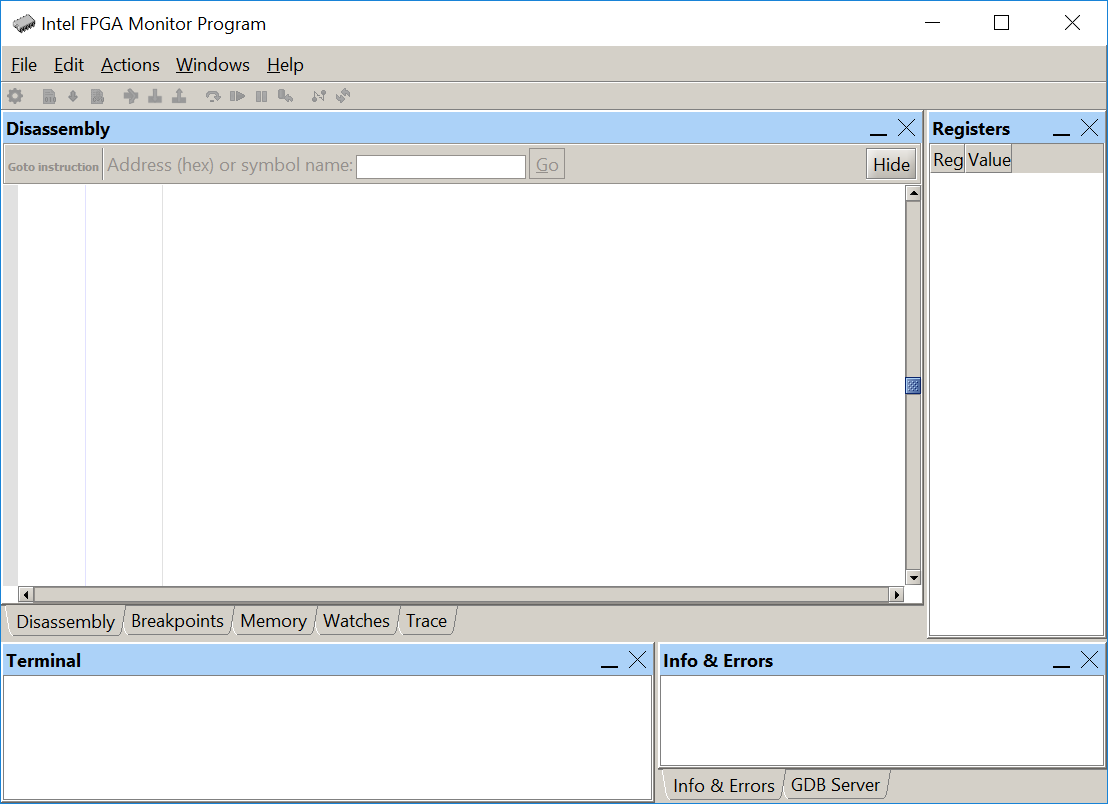
\includegraphics[scale=.67]{figures/figureMP1.png}
	\end{center}
	\caption{The \productNameMed{} window.}
\label{fig:MP1}
\end{figure}

\begin{figure}[H]
	\begin{center}
	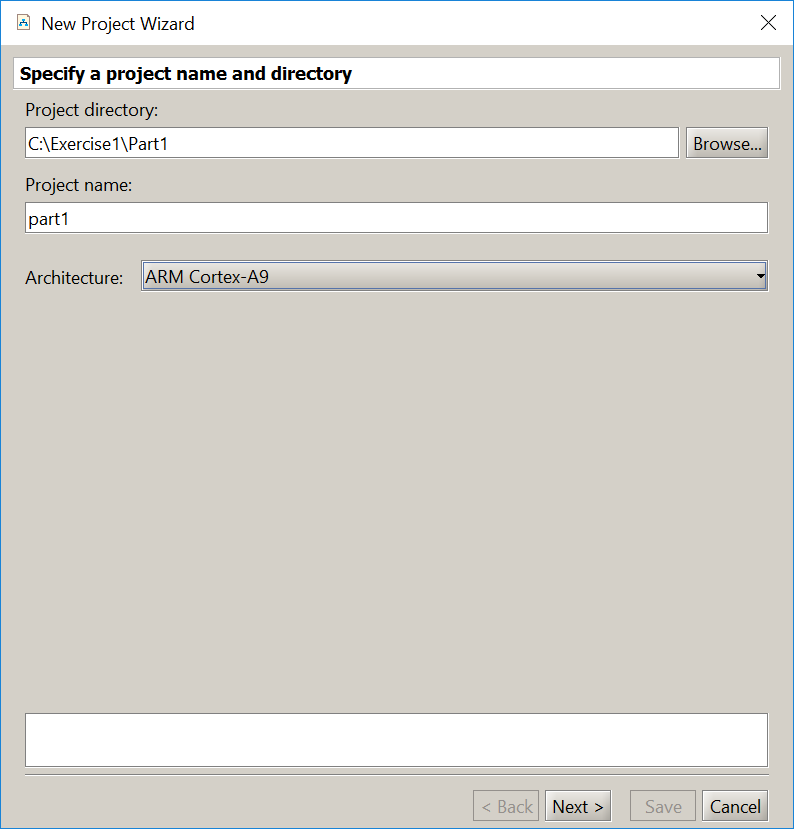
\includegraphics[scale=0.67]{figures/figureMP2.png}
	\end{center}
	\caption{Specify the folder and the name of the project.}
\label{fig:MP2}
\end{figure}

\begin{figure}[H]
	\begin{center}
	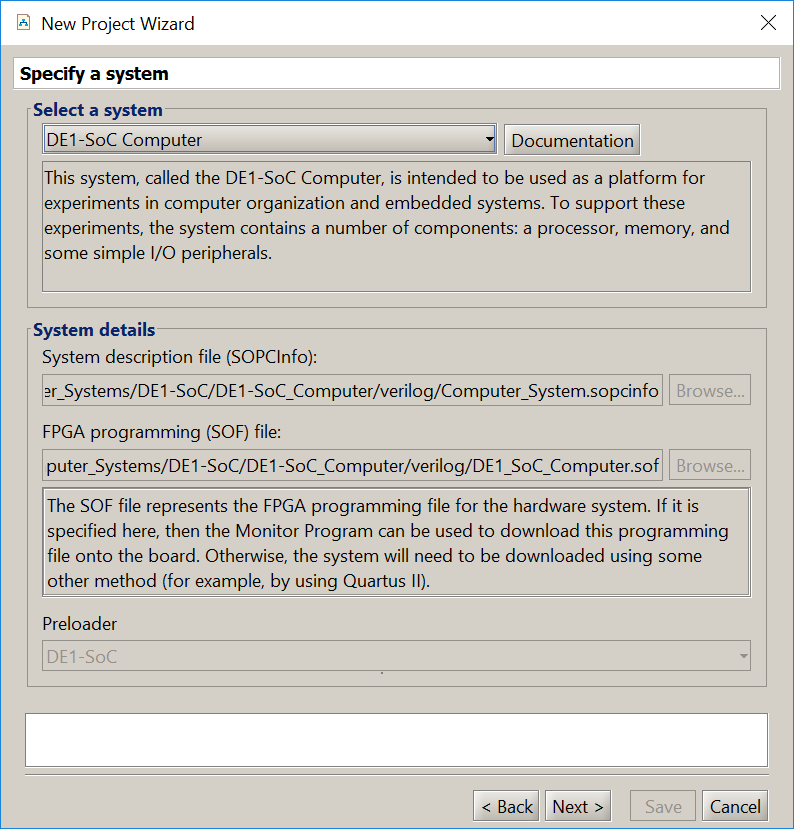
\includegraphics[scale=0.67]{figures/figureMP3.png}
	\end{center}
	\caption{Specification of the system.}
\label{fig:MP3}
\end{figure}

\item In the window in Figure~\ref{fig:MP4} you can specify the type of application 
programs that you wish to run. They can be written in either assembly language
or the C programming language.  Specify that an assembly language program will be used. 
The \productNameMed{} package contains several sample programs.
Select the box {\sf Include a sample program with the project}.
Then, choose the {\sf Getting Started} program, as indicated in the figure, and 
click {\sf Next}.

\item The window in Figure~\ref{fig:MP5} is used to specify the source file(s) that contain the
application program(s).
Since we have selected the {\it Getting Started} program, the window indicates the source
code file for this program. This window also allows the user to specify the starting point in the
selected application program. The default symbol is {\it \_start}, which is used
in the selected sample program. Click {\sf Next}. 

\item The window in Figure~\ref{fig:MP6} indicates some system parameters.
Note that the figure indicates that the {\it DE-SoC [USB-1]} cable is selected to provide 
the connection between the DE-series board and the host computer. This is the name assigned to the 
Intel USB-Blaster connection between the computer and the board.  Click {\sf Next}.

\begin{figure}[H]
	\begin{center}
	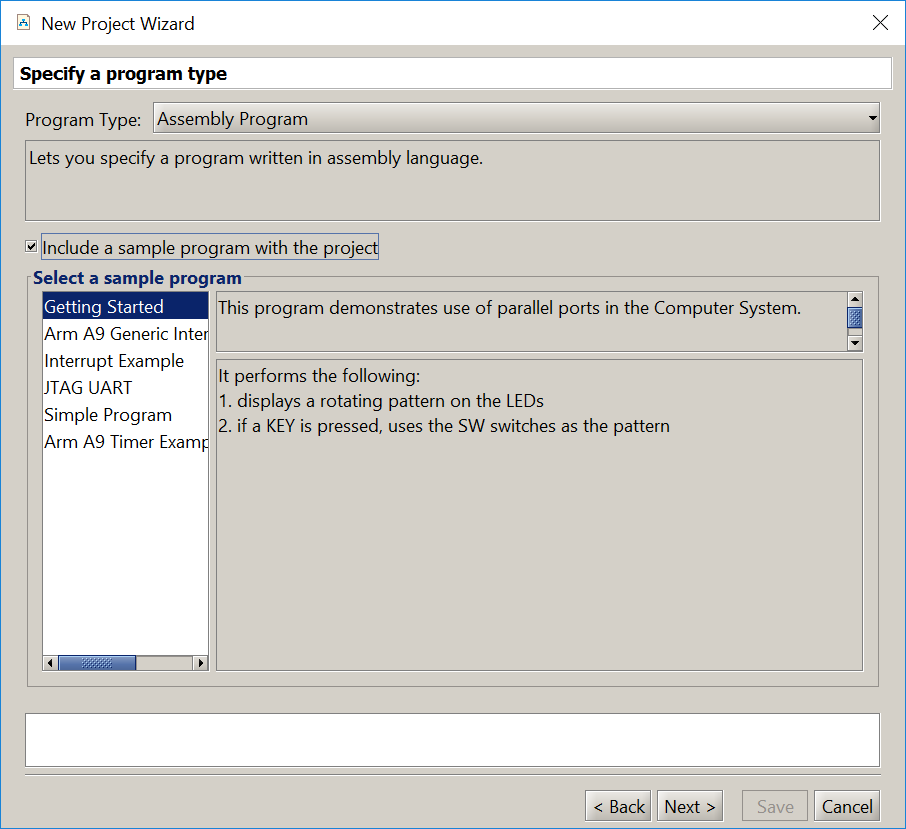
\includegraphics[scale=0.65]{figures/figureMP4.png}
	\end{center}
	\caption{Selection of an application program.}
\label{fig:MP4}
\end{figure}

\begin{figure}[H]
	\begin{center}
	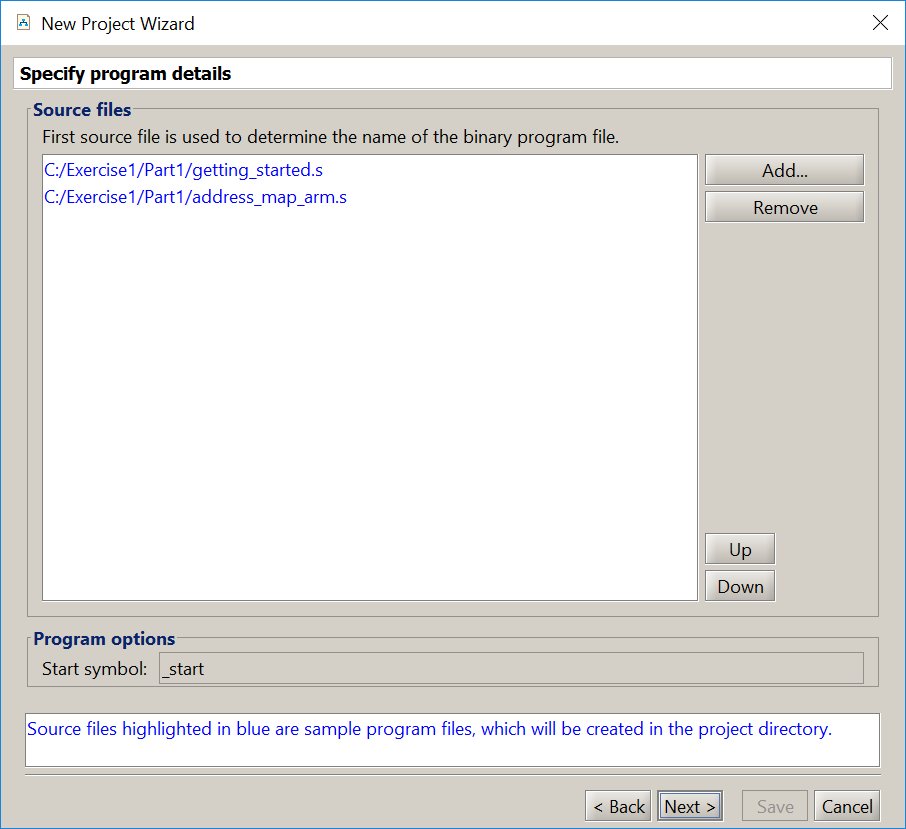
\includegraphics[scale=0.65]{figures/figureMP5.png}
	\end{center}
	\caption{Source files used by the application program.}
\label{fig:MP5}
\end{figure}

\begin{figure}[H]
	\begin{center}
	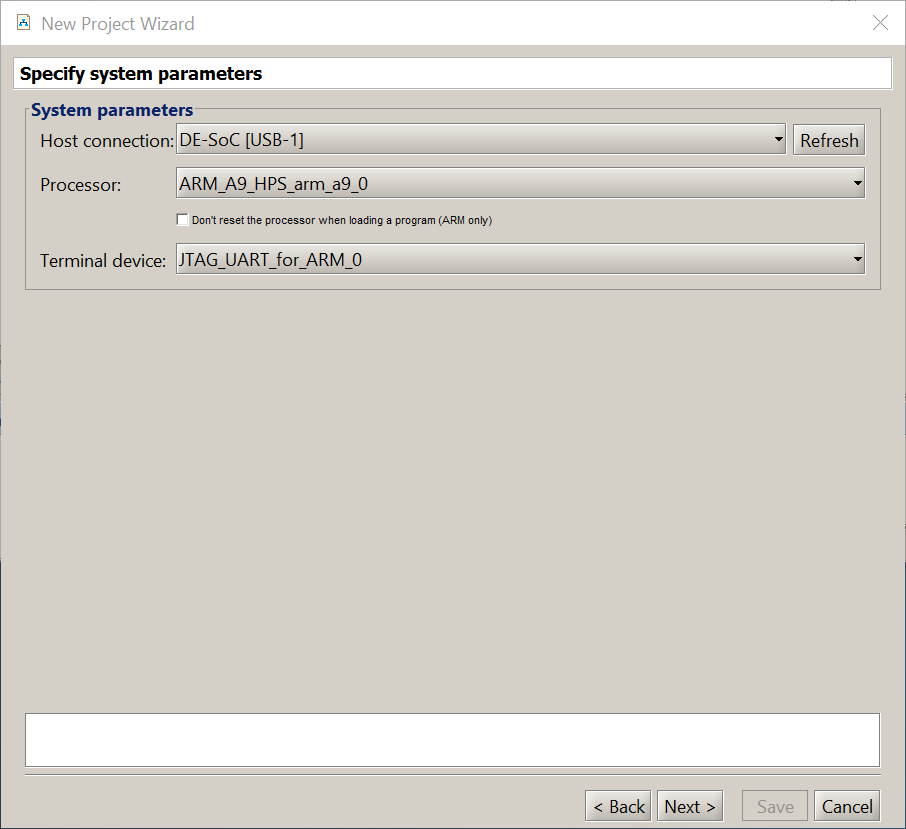
\includegraphics[scale=0.75]{figures/figureMP6.png}
	\end{center}
	\caption{Specify the system parameters.}
\label{fig:MP6}
\end{figure}

\item The window in Figure~\ref{fig:MP7} displays the names of Assembly sections that will
		  be used for the program, and allows the user to select a target memory location
		  for each section. In this case only the .{\it text} section, which corresponds to
		  the program code (and data), is defined. As shown in the figure, the .{\it text}
		  section is targeted to the DDR3 memory in the DE-series board, starting at
		  address 0. 
Click {\sf Finish} to complete the specification of the new project.

\item Since you specified a new project, a pop-up box will appear asking you if
you want to download the system associated with this project onto the DE-series board.
Make sure that the power to the board is turned on and click {\sf Yes}.
After the download is complete, a pop-up box
will appear informing you that the circuit has been successfully downloaded - click {\sf OK}.
If the circuit is not successfully downloaded, make sure that the USB connection, through 
which the USB-Blaster communicates, is established and recognized by the host computer. 
(If there is a problem, a possible
remedy may be to unplug the USB cable and then plug it back in.)

\begin{figure}[H]
	\begin{center}
	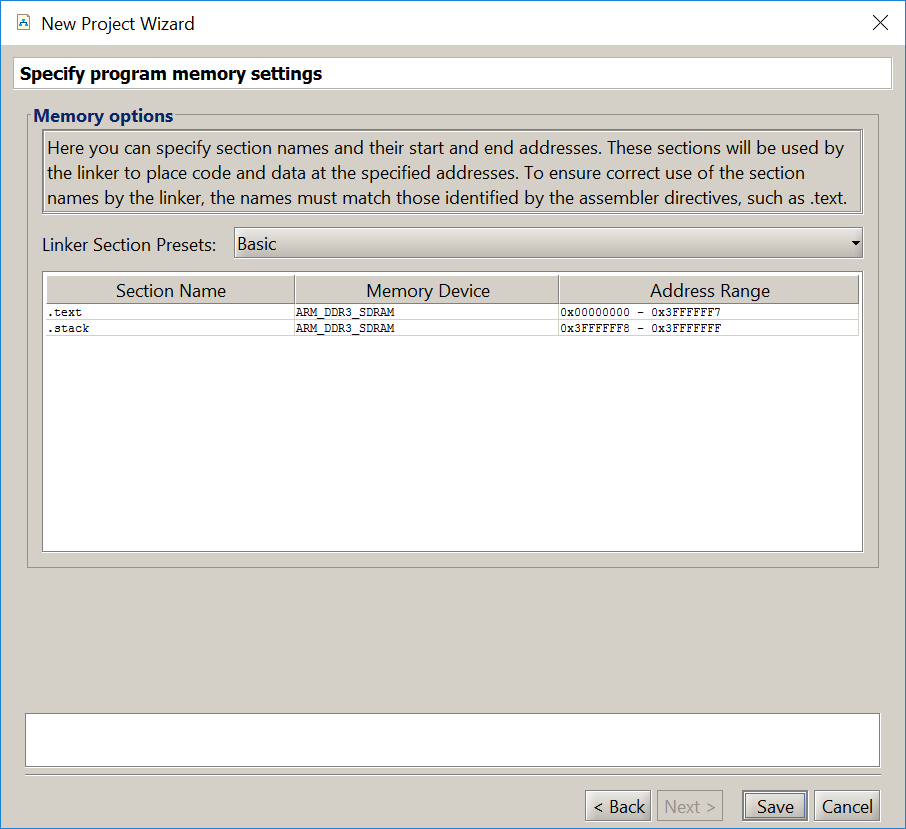
\includegraphics[scale=0.85]{figures/figureMP7.png}
	\end{center}
	\caption{Specify the program memory settings.}
\label{fig:MP7}
\end{figure}

\item Having downloaded the Computer into the Cyclone V SoC chip on your DE-series board, 
we can now load and run the sample program.
In the main Monitor Program window, shown in Figure~\ref{fig:MP9}, 
select {\sf Actions $>$ Compile \& Load} 
to assemble the program and load it into the FPGA chip.
Figure~\ref{fig:MP9} shows the Monitor Program window after the sample program has been loaded. 
\item Run the program by selecting {\sf Actions $>$ Continue} or
by clicking on the toolbar icon \hbox{
\includegraphics[scale=0.8]{figures/icon_continue.png}}, 
and observe the patterns displayed on the LEDs. 
\item Pause the execution of the sample program by clicking on the 
icon \hbox{
\includegraphics[scale=0.8]{figures/icon_pause.png}}, 
and disconnect from this session
by clicking on the icon \hbox{
\includegraphics[scale=0.8]{figures/icon_disconn.png}}, 

\begin{figure}[H]
	\begin{center}
	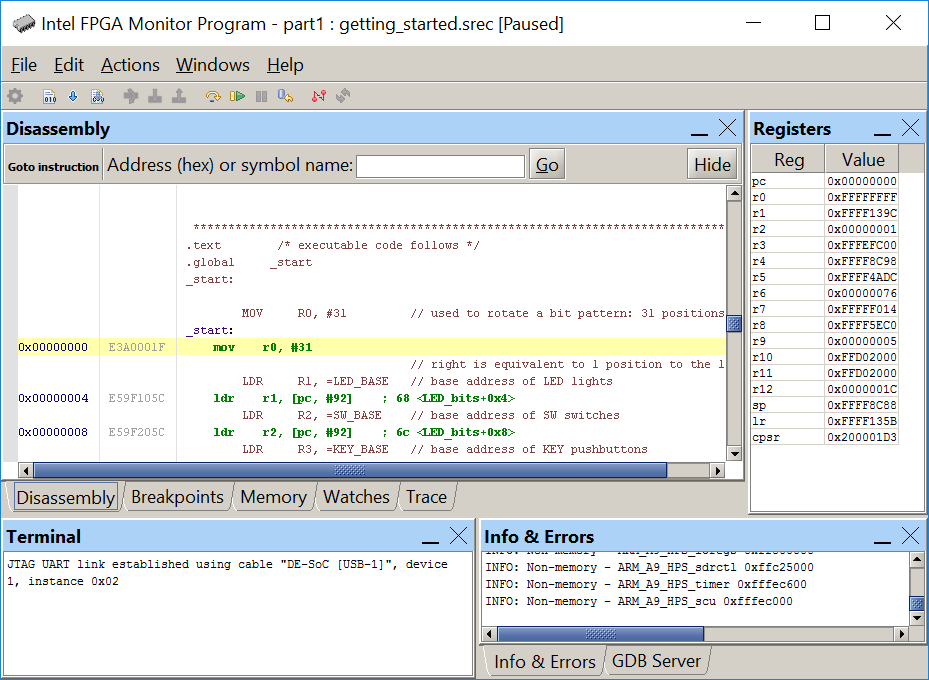
\includegraphics[scale=0.90]{figures/figureMP9.png}
	\end{center}
	\caption{The monitor window showing the loaded sample program.}
\label{fig:MP9}
\end{figure}

\end{enumerate}

\clearpage
\noindent
{\bf Part II}
~\\
~\\
\noindent
Now, we will explore some features of the Monitor Program by using a
simple application program written in the ARM assembly language.
Consider the program in Figure~\ref{fig:code}, which finds the largest number in a list
of 32-bit integers that is stored in the memory.

\begin{figure}[H]
\begin{center}
\lstinputlisting[style=defaultArmStyle]{../design_files/part2.s}
\end{center}
\caption{Assembly-language program that finds the largest number.}
\label{fig:code}
\end{figure}

~\\
\noindent
Note that some sample data is included in this program.
The word (4 bytes) at the label {\it RESULT} is reserved for storing the result, which will be 
the largest number found. The next word, $N$, specifies the number of entries in the list.
The words that follow give the actual numbers in the list.

~\\
\noindent
Make sure that you understand the program in Figure~\ref{fig:code} and the meaning of each 
instruction in it. Note the extensive use of comments in the program.
You should always include meaningful comments in programs that you will write!

~\\
\noindent
Perform the following:

\begin{enumerate}
\item Create a new folder for this part of the exercise, with a name such as {\it Part2}.  
Create a file named {\it part2.s} and enter the code from Figure~\ref{fig:code} into this
file.  Use the Monitor Program to create a new project in this folder; we have chosen the 
project name {\it part2}.  When you reach the window in Figure~\ref{fig:MP4} 
choose {\sf Assembly Program} but do not select a sample program. Click {\sf Next}.
\item Upon reaching the window in Figure~\ref{fig:MP5}, you have to specify the source
		  code file for your program.
Click {\sf Add} and in the pop-up box that appears indicate the desired file name,
{\it part2.s}.  Click {\sf Next} to get to the window in Figure~\ref{fig:MP6}. 
Again click {\sf Next} to get to the window in Figure~\ref{fig:MP7}. Notice that the 
DDR3\_SDRAM is selected as the memory device.  Your program will be loaded starting at
address 0 in this memory.  Click {\sf Finish}.
\item Compile and load the program.

\item The Monitor Program will display a disassembled view of the machine code loaded
in the memory, as indicated in Figure~\ref{fig:MP11}. 
Note that the pseudo instruction {\bf LDR R4, =RESULT} from your source code
has been implemented by using the instruction, {\bf LDR R4, [PC, \#84]}.
This instruction loads the 32-bit address of the label RESULT into register R4. 
After this instruction has been executed, the content of register R4 will be 
{\sf 0x00000038}, because this is the address in the memory of the label RESULT.

The {\bf LDR R4, [PC, \#84]} instruction loads the required 32-bit constant 
{\sf 0x00000038} from the {\it literal pool}, where this value has been placed by the 
assembler/linker. The address in the literal pool is calculated as [pc] + {\sf 8} + 
{\it OFFSET}, where {\it OFFSET}$ = ${\sf 0x54} in this case (84 in decimal). The reason 
that {\sf 8} is added has to do with the way that the ARM processor automatically
increments its program counter register as instructions are being executed.
Hence, the location in the literal pool where the processor gets the constant 
{\sf 0x00000038} in this case is {\sf 0} + {\sf 8} + {\sf 0x54} = {\sf 0x0000005C}.

You can use the Monitor Program Disassembly tab (or the Memory tab) to verify that the 
constant {\sf 0x00000038} is in the literal pool at the address {\sf 0x0000005C}. 
Figure~\ref{fig:MP12} shows the literal-pool constant in the Disassembly window.
You can single-step the instruction {\bf LDR R4, =RESULT} in the Monitor Program to verify
that it sets R4 to the value {\sf 0x00000038}.

\item Execute the program. When the code is running, you will not be able to see any changes
(such as the contents of registers or memory locations) in the Monitor Program window,
because the Monitor Program cannot communicate with the ARM processor while code is being
executed.  But, if you pause the program then the Monitor Program window will be updated.
Pause the program using the icon \hbox{
\includegraphics[scale=0.8]{figures/icon_pause.png}}
and observe that the processor stops within the endless loop {\bf END: B END}.
Note that the largest number found in the sample list is 8 as indicated
by the contents of register R0. This result is also stored in memory at the label
RESULT.  As discussed above, the address of the label RESULT for this program is {\sf 0x00000038}.
Use the Monitor Program's Memory tab, as illustrated in Figure~\ref{fig:MP_mem},
to verify that the resulting value 8 is stored in the correct location.

\item You can return control of the program to the start by clicking 
		  on the icon \hbox{
\includegraphics[scale=0.8]{figures/icon_restart.png}}, or by
		  selecting {\sf Actions} $>$ {\sf Restart}. 
Do this and then single-step through the program by clicking on the icon
\hbox{
\includegraphics[scale=0.8]{figures/icon_step.png}}. Watch how the instructions change the 
data in the processor's registers.

\item Double-click on the {\sf pc} register in the Monitor Program and then set the program
counter to 0. Note that this action has the same effect as
clicking on the restart icon \hbox{
\includegraphics[scale=0.8]{figures/icon_restart.png}}. 

\item Now set a breakpoint at address {\sf 0x0000002C} by clicking on the gray bar to
the left of this address, as illustrated in Figure~\ref{fig:MP13}. Restart the program and run 
it again.  Observe the contents of register R0 each time the instruction at the
breakpoint, which is \texttt{B LOOP}, is reached.

\begin{figure}[H]
	\begin{center}
	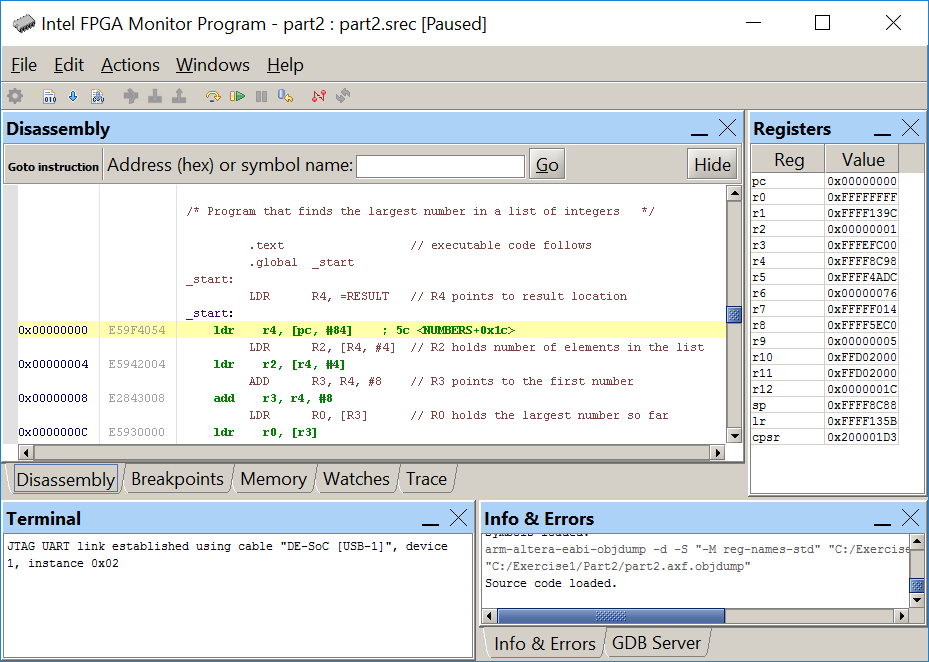
\includegraphics[scale=0.8]{figures/figureMP11.png}
	\end{center}
	\caption{The disassembled view of the program in Figure~\ref{fig:code}.}
\label{fig:MP11}
\end{figure}

\begin{figure}[H]
	\begin{center}
	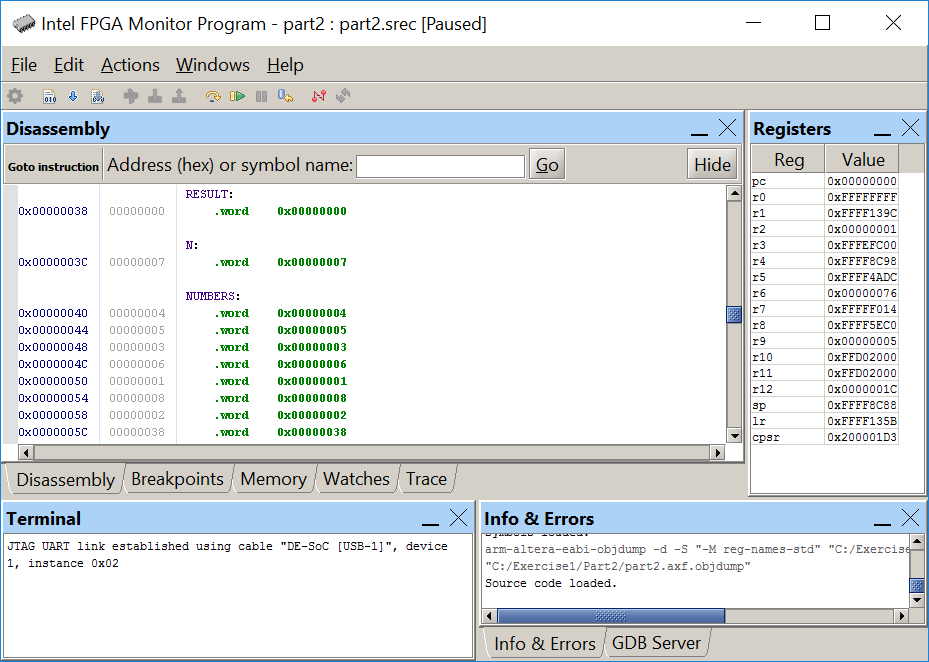
\includegraphics[scale=0.8]{figures/figureMP12.png}
	\end{center}
	\vspace{-0.5cm}\caption{The constant {\sf 0x00000038} in the literal pool at address
	{\sf 0x0000005C}.}
\label{fig:MP12}
\end{figure}

\begin{figure}[H]
	\begin{center}
	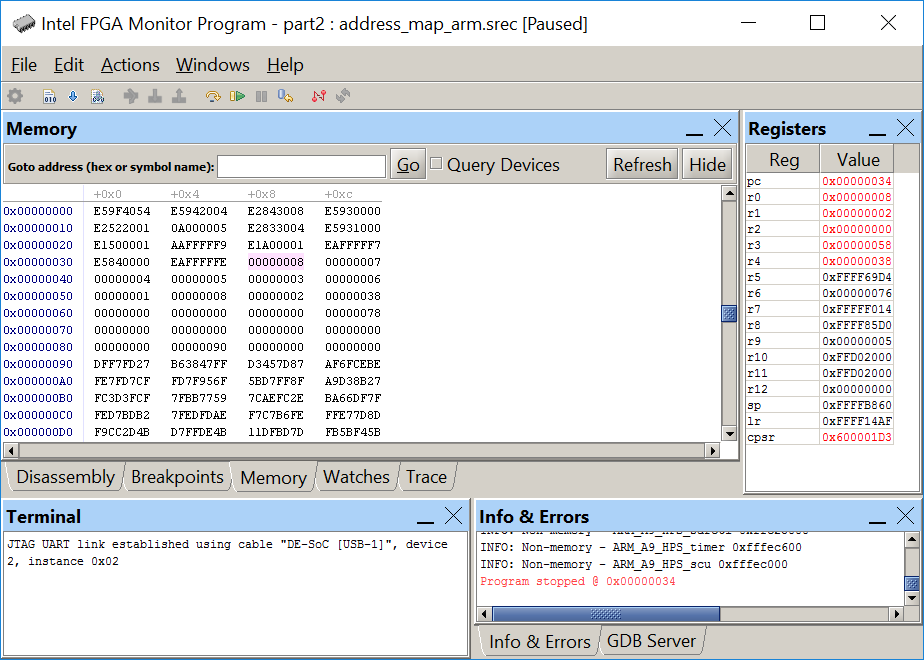
\includegraphics[scale=0.8]{figures/figureMP_mem.png}
	\end{center}
	\vspace{-0.5cm}\caption{Displaying the result in the memory tab.}
\label{fig:MP_mem}
\end{figure} 

\begin{figure}[H]
	\begin{center}
	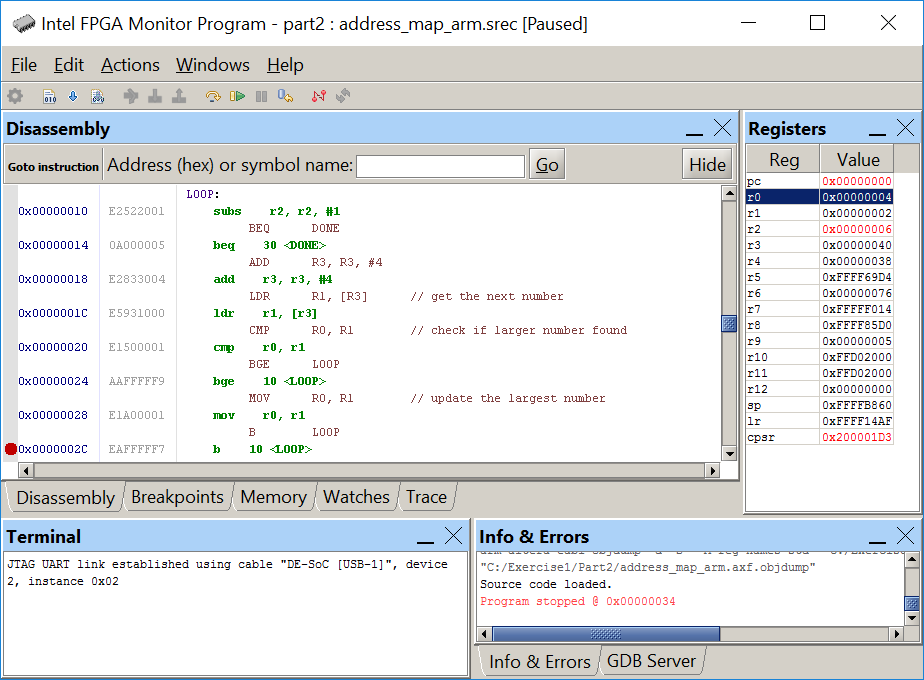
\includegraphics[scale=0.8]{figures/figureMP13.png}
	\end{center}
	\vspace{-0.5cm}\caption{Setting a breakpoint.}
\label{fig:MP13}
\end{figure} 

\end{enumerate}

\newpage
\noindent
{\bf Part III}

~\\
\noindent
Implement the task in Part II by modifying the program in Figure~\ref{fig:code} so that it
uses a subroutine. The subroutine, LARGE, has to find the largest number in a list.
The main program passes the number of entries and the address of the start of the
list as parameters to the subroutine via registers R0 and R1.
The subroutine returns the value of the largest number to the calling program
via register R0. A suitable main program is given in Figure~\ref{fig:main}.
~\\

\noindent
Create a new folder and a new Monitor Program project to compile and download your program.
Run your program to verify its correctness.

\begin{figure}[H]
\begin{center}
\lstinputlisting[style=defaultArmStyle]{../design_files/part3.s}
\end{center}
\caption{Main program for Part III.}
\label{fig:main}
\end{figure}

~\\
\noindent
{\bf Part IV}

~\\
\noindent
The program shown in Figure~\ref{fig:decimal} converts a binary number into two decimal digits.
The binary number is loaded from memory at the location $N$, and the two
decimal digits that are extracted from $N$ are stored into memory in two bytes starting at 
the location {\it Digits}. For the value $N = 76$ ({\sf 0x4c}) shown in the figure, the code sets 
{\it Digits} to {\sf 00000706}.

~\\
\noindent
Make sure that you understand how the code in Figure~\ref{fig:decimal} works. Then, extend
the code so that it converts the binary number to four decimal digits, supporting decimal 
values up to 9999. You should modify the DIVIDE subroutine so that it can use any divisor, 
rather than only a divisor of 10. Pass the divisor to the subroutine in register R1.

~\\
\noindent
If you run your code with the value $N = 9876$ ({\sf 0x2694}), then {\it Digits} should be set to 
{\sf 09080706}.

\begin{figure}[H]
\begin{center}
\lstinputlisting[style=defaultArmStyle]{../design_files/part4.s}
\end{center}
\caption{A program that converts a binary number into two decimal digits.}
\label{fig:decimal}
\end{figure}


%%%%%%%%%%%%%%%%%%%%%%%%%%%%%%%%%%%%%%%%
%%% FPGAcademy Copyright Information %%%
%%%%%%%%%%%%%%%%%%%%%%%%%%%%%%%%%%%%%%%%

%Always put the copyright on a new page (clear page), with some vertical space from top
\clearpage
\vspace{1in}

\noindent

Copyright {\copyright} FPGAcademy.org. All rights reserved. FPGAcademy and the 
FPGAcademy logo are trademarks of FPGAcademy.org.  This document is provided 
"as is", without warranty of any kind, express or implied, including but not 
limited to the warranties of merchantability, fitness for a particular purpose 
and noninfringement. In no event shall the authors or copyright holders be 
liable for any claim, damages or other liability, whether in an action of 
contract, tort or otherwise, arising from, out of or in connection with the 
document or the use or other dealings in the document.
~\\
~\\
**Other names and brands may be claimed as the property of others.


\end{document}
